\documentclass[12pt, a4paper]{article}
\usepackage{graphicx}
\graphicspath{ {./images/} }
\usepackage{subcaption}
%\usepackage{tipa}
\setlength{\oddsidemargin}{0.5cm}
\setlength{\evensidemargin}{0.5cm}
\setlength{\topmargin}{-1.6cm}
\setlength{\leftmargin}{0.5cm}
\setlength{\rightmargin}{0.5cm}
\setlength{\textheight}{24.00cm} 
\setlength{\textwidth}{15.00cm}
\parindent 0pt
\parskip 5pt
\pagestyle{plain}

\title{Master Thesis Proposal}
\author{Kefang Ding} 
\date{\today}

\newcommand{\namelistlabel}[1]{\mbox{#1}\hfil}
\newenvironment{namelist}[1]{%1
\begin{list}{}
    {
        \let\makelabel\namelistlabel
        \settowidth{\labelwidth}{#1}
        \setlength{\leftmargin}{1.1\labelwidth}
    }
  }{%1
\end{list}}

\begin{document}
\maketitle
\hrulefill
\begin{namelist}{xxxxxxxxxxxx}
\item[{\bf Title:}]
	Process Enhancement by Incorporating Negative Information in Model Repair
\item[{\bf Author:}]
	Kefang Ding
\item[{\bf Supervisor:}]
    Professor Dr. ir. Wil van der Aalst
    \newline
	Dr. ir. Sebastiaan J. van Zelst

\item[{\bf Degree:}]
	Master of Science
\end{namelist}
\hrulefill 

\section*{Introduction} 

Process mining techniques aim to support the analysis of business processes based on event logs. These techniques focus on three tasks: process discovery, conformance checking and model enhancement. Process discovery aims to discover a new model from an event log in order to understand the business process execution. Conformance checking analyzes the deviation between process models and observed behavior during execution. Enhancement improves an existing model based on an event log by extending the model with more data perspectives or repairing the existing model to better reflect observed behaviors.  

Between those techniques, repair model belongs to process enhancement and stands between process discovery and conformance checking. It improves the existing model by adding loops, subprocess, and removing infrequent transitions \cite{Fahland}. Later in \cite{Dees} \cite{Anja}, focuses are not only on fitness improvement but also on good KPI outcomes. However, the state-of-the-art model repair methods only consider the positive information which benefits the good performance, but leave out the impact from negative information. It usually results in a less precise model, which can be shown in the following example.
 
The original model is defined in the Figure \ref{fig:model_examples} (a), where A is followed directly by B. During its execution in real life, an event log is generated: \[{ <A, B> }^{55}  , {<B, A>}^{105} \] 
After current model repair techniques in \cite{Anja}\cite{Dees}, a new process model with high fitness is generated. A and B now have parallel relation. 
If we analyze the impact on performance according to KPI, the event log is divided into positive and negative set: 
\[ Positive \;  examples: { <A, B> }^{5}  , {<B, A>}^{100} \] 
\[ Negative \; examples: { <A, B> }^{50}  , {<B, A>}^{5} \]  
Under consideration of only positive information, the repaired model keeps the same like in Figure \ref{fig:model_examples}(b), since both $<A,B> and <B,A>$ contributes to good performance. 

\begin{figure}[h]
	\centering
	\begin{subfigure}[b]{0.32\textwidth}
		\centering
		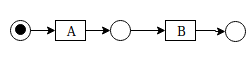
\includegraphics[width=\linewidth]{P04_modelchange_a.png}
		\caption{original process model}
		\label{fig:model_a}
	\end{subfigure}
\hfill
	\begin{subfigure}[b]{0.32\textwidth}
		\centering
	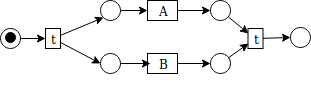
\includegraphics[width=\linewidth]{P04_modelchange_b.png}
	\caption{process model \\ with high fitness}
	\label{fig:model_b}
\end{subfigure}
\hfill
	\begin{subfigure}[b]{0.32\textwidth}
		\centering
	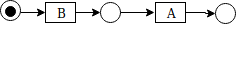
\includegraphics[width=01.0\linewidth]{P04_modelchange_c.png}
	\caption{process model \\ with good KPI}
	\label{fig:model_c}
\end{subfigure}

	\caption{example for model change under model repair}
	\label{fig:model_examples}
\end{figure}

However, it's obvious that $<A,B>$ leads to more bad performance than good ones and should be avoided. The Figure \ref{fig:model_examples}(c) shows the expected model with incorporating the negative information. This model reinforces positive examples and avoids negative examples, which provides us a better business execution process.

On the other side, the current methods in \cite{Anja}\cite{Dees} are not capable to combine multiple KPI at the same time, which leads the generation of good model difficult.

\section*{Aim}
Given input of one existing process model, an event log and KPIs, our aim is to improve current process enhancement techniques by incorporating negative information within process model repair, and generate a better  process model with higher fitness, precision and better KPIs outcomes. Therefore, the repaired model provides a better way to understand and execute the real business process.

To evaluate the improvement, we will build a confusion matrix in the Table \ref{table:confusion_matrix}. The columns represent model allowed behavior and not allowed behavior; the rows means the positive examples and negative ones in the event log.  Good improvement should increase the diagonal ratio in the table, namely the AP and NN, while lowering the percentage of reverse diagonal, which is PN and AN.
\begin{table}[h!]
	\centering
	\caption{confusion matrix for evaluation}
	\label{table:confusion_matrix}
\begin{tabular}{|l|l|l|}
	\hline
	&	Allowed behavior & 	Not allowed behavior \\
	\hline
	Positive Examples  &	AP & 	PN \\	
	\hline
	Negative Examples    &	AN & 	NN \\	
	\hline
\end{tabular}
\end{table}

% by building recall or precision, I could compare it with other methods to create the confusion matrix.
Under the current techniques for repair model, only positive example are considered and the model in the middle is generated. In the view of its confusion matrix in Table \ref{table:confusion_matrix}, it has less precision by allowing all behavior in model.
\begin{table}[h!]
\centering
\caption{confusion matrix for given example in current approach}
\label{table:cm_current}
\begin{tabular}{|l|l|l|}
	\hline
	&	Allowed behavior & 	Not allowed behavior \\
	\hline
	Positive Examples  &	105 & 	0 \\	
	\hline
	Negative Examples    &	55 & 	0 \\	
	\hline
\end{tabular}
\end{table}

%The evaluation result is ??? 


% put table together and then give the evaluation value. 
In our approach, both negative and positive examples are used to generate expected model. The confusion matrix is driven in Table \ref{table:cm_improved}. 
\begin{table}[h!]
	\centering
	\caption{confusion matrix for given example in improved approach}
	\label{table:cm_improved}
\begin{tabular}{|l|l|l|}
	
	\hline
	&	Allowed behavior & 	Not allowed behavior \\
	\hline
	Positive Examples  &	100 & 	5 \\	
	\hline
	Negative Examples    &	5 & 	50 \\	
	\hline
\end{tabular}
\end{table}

%The evaluation result is ?? 

Also, given multiple KPIs, it should be able to combine them together and provide a balanced model with good performance. But this suggestion should be based on the hypothesis:
 
\section*{Method}
The inputs for process model enhancement within model repair includes the following data:
\begin{itemize}
	\item Existing process modeled using Petri net
	\item Event Log corresponding the actual execution of modeled process
	\item Key Performance Indicators(KPIs)
\end{itemize}
 Our approach produces a repaired model as output and its workflow is shown in the Figure \ref{fig:approach}. The first phase in shadow accepts an existing process and an event log as input, then repairs model w.r.t. fitness.  After that the event log is classified into positive and negative examples w.r.t. KPIs, both positive and negative examples are passed to the second phase besides the repaired model with good fitness. At last, the model is modified to reinforce the good examples while avoiding the negative examples in event log. 
\begin{figure}[h!]
	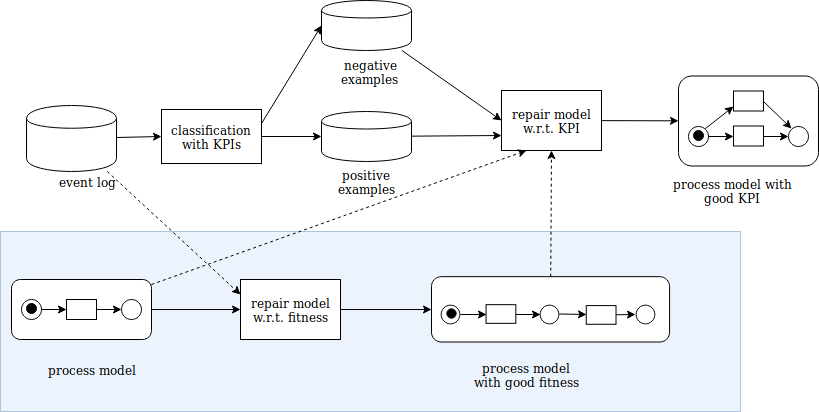
\includegraphics[width=\textwidth]{P04_approach.png}
	\caption{our approach to repair model}
	\label{fig:approach}
\end{figure}

The first phase is optional, if the process model has good fitness, it is passed directly to the phase to repair model w.r.t. KPI. If not, we use the model repair framework in \cite{Fahland}. Subprocess and loops are inserted into the original model. Infrequent paths are removed later to keep the model with good fitness and better precision. 

To classify the event log with KPIs, decision tree, associated rules are used.Later, another improvement of the approach can be introduced to combine multiple KPIs, and quantify the goodness of event trace. However, it is based on the following hypothesis. 
\begin{itemize}
	\item By implying the quantitative impact from multiple KPIs on model repair, we could get better result than by only using the classification method.  
\end{itemize} 

Now, to incorporate negative information on model improvement, we are motivated from \cite{pesic} \cite{Broucke} \cite{Lamma} \cite{chesani} which uses Inductive Logic Programming techniques like TILDE or SCIFF to get model constraints from positive and negative examples. Based on this, we propose our own method to repair model. 
\begin{itemize}
	\item change Petri net into rules constraints.\\
	Business Process in Petri net imposes  the (minimal) set
	of constraints that must be satisfied when executing the process activities. Thoese constraints can be expressed into a declarative language like ConDec. 
	\item train rules based on the positive and negative examples and get modified rules. \\ 
	After the transformation from Petri net, we have the set of existing constraints which enable both the positive and negative performance. By using ILP techniques, we can find a set of rules under the current existing constraints, which separates the given positive and negative examples.
	\item transform the modified rules again into Petri net\\
	Improved Constraints on business process are used to generate a new Petri net.
\end{itemize}
To make sure the method above feasible, several hypotheses are needed: 
\begin{enumerate}
	\item The mapping from Petri net patterns and the rules in first-order logic is possible and bijective, such that the two-sided transformation is feasible.
	\item Generated model considers the impact from positive and negative examples but still keeps the similarity to the original model. 
\end{enumerate}

The next primary work should test on the hypotheses. 


\section*{Software and Hardware Requirements}

The platform is ProM6, a open source project for process mining. To implement our approach, those plugins are in demand. 
\begin{itemize}
	
	\item  repair w.r.t. fitness 
	
	   Repair Model in Uma package
	\item repair w.r.t. KPI
	   \subitem	   Inductive Logic Programming
	   \subitem	   Decision Tree : weka
	   \subitem	   Associated Rules : weka
	   \subitem    Regression function : weka
\end{itemize}


\section*{Timeline}
The original plan for our project is in the table listed below.
\begin{table}[h!]
	\caption{ time line for the work}
\begin{tabular}{|l|l|}
	\hline time & taks \\
\hline August &
Test the proposed hypotheses by creating small demo \\
\hline September &
Register master thesis and design the architecture \\
\hline October &
Coding and debug \\
\hline November &
 Test and Write Thesis \\
\hline December &
Write thesis and representation \\
\hline
\end{tabular}
\end{table}

\begin{thebibliography}{9}
\bibitem{Fahland} Fahland, Dirk, and Wil MP van der Aalst. "Model repair—aligning process models to reality." Information Systems 47 (2015): 220-243.
\bibitem{Dees} Dees, Marcus, Massimiliano de Leoni, and Felix Mannhardt. "Enhancing process models to improve business performance: a methodology and case studies." OTM Confederated International Conferences" On the Move to Meaningful Internet Systems". Springer, Cham, 2017.
\bibitem{Anja} Adriansyah, Arya, et al. "Alignment based precision checking." International Conference on Business Process Management. Springer, Berlin, Heidelberg, 2012.
\bibitem{Broucke} vanden Broucke, Seppe KLM, et al. "Determining process model precision and generalization with weighted artificial negative events." IEEE Transactions on Knowledge \& Data Engineering 1 (2013): 1.
\bibitem{Buijs}Buijs, Joos CAM, et al. "Improving business process models using observed behavior." International Symposium on Data-Driven Process Discovery and Analysis. Springer, Berlin, Heidelberg, 2012.
\bibitem{Lamma} Montali, Marco, et al. "Declarative specification and verification of service choreographiess." ACM Transactions on the Web (TWEB) 4.1 (2010): 3.
\bibitem{pesic} Pesic, Maja, and Wil MP Van der Aalst. "A declarative approach for flexible business processes management." International conference on business process management. Springer, Berlin, Heidelberg, 2006.
\bibitem{lamma} Lamma, Evelina, et al. "Applying inductive logic programming to process mining." International Conference on Inductive Logic Programming. Springer, Berlin, Heidelberg, 2007.
\bibitem{chesani} Chesani, Federico, et al. "Exploiting inductive logic programming techniques for declarative process mining." Transactions on Petri Nets and Other Models of Concurrency II. Springer, Berlin, Heidelberg, 2009. 278-295.
\end{thebibliography}


\end{document}

